\chapter{THE COMING LIBERTARIAN AGE \\古典自由主义时代来临了}
\begin{paracol}{2}
\hbadness5000

In 1995 Gallup pollsters found that 39 percent of Americans said that ``the federal government has become so large and powerful that it poses an immediate threat to the rights and freedoms of ordinary citizens.'' Pollsters couldn't believe it, so they tried again, taking out the word ``immediate.'' This time 52 percent of Americans agreed.

\switchcolumn
1995年,盖勒普调查发现,39\%的美国人认为“联邦政 府规模和权力过大,以至于产生了对普通公民自由和权利的直接威胁”。调查人员对这个结果难以置信,于是他们重新做了调查,把“直接”两个字去掉。这回的结果是52\% 。

\switchcolumn*
Later that year \textit{USA Today} reported in a front-page story on
post-baby-boom Americans that ``many of the 41 million members of Generation X$\ldots$ are turning to an old philosophy that suddenly seems new: libertarianism.'' A front-page report in the \textit{Wall Street Journal} agreed: ``Much of the angry sentiment coursing through [voters'] veins today isn't traditionally Republican or even conservative. It's libertarian$\ldots$ Because of their growing disdain for government, more and more Americans appear to be drifting---often unwittingly---toward a libertarian philosophy.''

\switchcolumn
同年晚些时候,《今日美国》在一个关于婴儿潮时代美国 人的封面专题中报道说:“100万的‘X一代人’\footnote{“X一代人” ,这个词首先是由美国的《时代》 杂志提出来的,他们在1990年7月16日的封面文章中把出生于20世 纪 60年代中期到70年代末的年轻人称作“X一代”。}当中的很多人 $\cdots \cdots$ 正在倾向于一种虽然古老,却突然显得很现代的理论:古典自由主义。” 《华尔街日报》在一篇封面报道中也同意这个观点:“如今在选民当中涌动的愤怒情绪与传统的共和 党甚至保守主义无关,而是古典自由主义 $\cdots \cdots$ 由于他们对政府 的不满不断增长,越来越多的美国人开始转向古典自由主义理论,尽管这种转向常常是无意识的。”

\switchcolumn*
Writing in 1995 about the large numbers of Americans who say they'd welcome a third party, David Broder of the \textit{Washington Post} commented,

\switchcolumn
《华盛顿邮报》的大卫$\cdot$布罗德尔(David Broder) 也在 1995年的一篇文章中提到,相当多的美国人说他们欢迎第三党的出现,他说:

\switchcolumn*
\begin{quote}
	The distinguishing characteristic of these potential independent voters---aside from their disillusionment with Washington politicians of both parties---is their libertarian streak. They are skeptical of the Democrats because they identify them with big government. They are wary of the Republicans because of the growing influence within the GOP of the religious right.
\end{quote}


\switchcolumn
\begin{quote}
	这些独立选民---即那些对华盛顿的两大政党大失所望的选民---的一个鲜明特征就是他们的古典自由主义倾向。他们对民主党不信任,因为他们认为民主党主张大政府。他们也区别于共和党,因为共和党内对宗教权利的干预在不断增强。
\end{quote}
\switchcolumn*

Where did this sudden media interest in libertarianism
come from? As \textit{USA Today} noted, libertarianism challenges the
conventional wisdom and rejects outmoded statist ideas, so it
often has a strong appeal to young people. As for myself, when
I first discovered libertarian ideas in my college days, it seemed
obvious to me that most libertarians would be young (even
though I was dimly aware that the libertarian books I was
reading were written by older people). Who but a young person could believe in such a robust vision of individual freedom?
When I went to my first libertarian event off-campus, I was
mildly surprised that the first person I encountered was about
forty, which seemed quite old to me at the time. Then another
person arrived, more the sort of person I had expected to meet,
a young woman in her late twenties. But her first question was,
``Have you seen my parents?'' I soon learned that her sixtyish
parents were the leading libertarian activists in the state, and
my mistaken impressions about what kind of people would become libertarians were gone forever. I discovered that the
young woman's parents, and the millions of Americans who
today share libertarian beliefs, stand firmly in a long American
tradition of individual liberty and opposition to coercive government.

\switchcolumn
这些媒体为什么突然对古典自由主义兴趣盎然呢?正如
《今日美国》所说:古典自由主义对公众的因袭观念提出了挑
战,反对过时的国家主义的理念,因此对年轻人产生了强烈的
吸引力。拿我自己来说,当我在大学时期第一次接触到古典自
由主义理念的时候,我想当然地认为绝大多数古典自由主义者
应该很年轻(尽管我多少知道我所读的古典自由主义的著作
是由一些老人家写的)。除了年轻人谁还会信仰这种对个人自
由有着如此健全的洞察力的理论?当我第一次参加校外的古典
自由主义活动的时候,相当惊讶地看到我第一个碰到的家伙有
40岁左右,在当时的我看来这个年龄已经相当老了。然后,
另一个人进来了,一个20多不到30岁的年轻女人,这大约符
合我平时想像中这个群体的人应有的年龄段。然而,她看到我
之后问我的第一个问题却是: “你看到我爸妈了吗?”我很快
知道了她父母是这个州古典自由主义活动的组织者,而我关于
古典自由主义者应该是哪一类人的错误印象也就随之永远消失
了。我逐渐了解到,这个年轻女人的父母以及数以百万计信仰
古典自由主义的美国人,都坚定地站在一个悠久的美国传统一
边 ,那就是:坚持个人自由,反对政府强制。

\switchcolumn*
Libertarianism is the view that each person has the right to
live his life in any way he chooses so long as he respects the
equal rights of others. (Throughout this book I use the traditional ``he'' and ``his'' to refer to all individuals, male and female;unless the context indicates otherwise, ``he'' and ``his'' should be understood to refer to both men and women.) Libertarians defend each person's right to life, liberty, and property--rights that people possess naturally, before governments are created.
In the libertarian view, all human relationships should be voluntary; the only actions that should be forbidden by law are those that involve the initiation of force against those who have not themselves used force---actions like murder, rape, robbery, kidnapping, and fraud.
\switchcolumn
古典自由主义的基本理念是:每个人有权按照自己选择的
方式来生活,同时他也尊重别人的同样权利(在本书中,我
将使用传统的“他” 和 “他的”这两个代词来指代所有的个
人,无论男性还是女性;除非文中有特指,否 则 “他” 或
“他的” 应当理解为既指男人也指女人)。古典自由主义者捍
卫每个人的生命权、自由和财产权,即那些在政府产生之前人们就自然拥有的权利。在古典自由主义者看来,所有人与人的
关系都应该基于自愿;唯一应当被法律禁止的行为是那些对没
有使用暴力的人使用暴力的行为 --- 例如谋杀、强奸、抢劫、
绑架以及诈骗。

\switchcolumn*
Most people habitually believe in and live by this code of
ethics. Libertarians believe this code should be applied consistently--and specifically, that it should be applied to actions by
governments as well as by individuals. Governments should
exist to protect rights, to protect us from others who might use
force against us. When governments use force against people
who have not violated the rights of others, then governments
themselves become rights violators. Thus libertarians condemn
such government actions as censorship, the draft, price controls, confiscation of property, and regulation of our personal
and economic lives.
\switchcolumn
当然,绝大多数人基于习惯和常识相信这种道德准则,并
且按照这种准则来生活。但古典自由主义更相信这种准则应当
被一以贯之地遵循,政府尤其如此,这种准则应该像应用在个
人身上一样应用在政府行为上。政府的存在应该是为了保护我
们的权利,保护我们的权利不受到来自其他人的暴力侵害。当
政府对那些没有侵犯别人权利的个人使用暴力的时候,政府本
身就成了权利的侵害者。因此,古典自由主义者对诸如信息审
查 、强制征兵、价格管制、征用财产以及对我们个人和经济生
活的管制等政府行为会表示谴责。
\switchcolumn*
Put so starkly, the libertarian vision may sound otherworldly,
like a doctrine for a universe of angels that never was and never
will be. Surely, in today's messy and often unpleasant world,
government must do a great deal? But here's the surprise: The
answer is no. In fact, the more messy and modern the world,
the better libertarianism works compared--for instance--with
monarchy, dictatorship, and even postwar American-style welfarism. The political awakening in America today is first and
foremost the realization that libertarianism is not a relic of the
past. It is a philosophy---more, a pragmatic plan---for the future. In American politics it is the leading edge--not a backlash, but a vanguard.
\switchcolumn
看上去,古典自由主义的愿景也许有些空想,就像那种由
天使组成的世界里的教义一样,而那种天使世界从来都没有存
在过,将来也不会出现。那么,在今天这个混乱而糟糕的世界
上,政府是不是有很多工作要做?答案是意外的:不是。事实
上 ,这个世界越是混乱和现代,古典自由主义与君主制和独裁
体制相比就越有效,甚至比战后美国的福利主义体制更有效。
在当今美国,政治上最重大的进展是意识到古典自由主义并不
是旧时代的文物,而是一种面向未来的理论和现实的可操作的
计划。在美国政治当中它是一种领导力量 --- 不是一种复辟,
而是一种先锋的力量。

\switchcolumn*
Libertarian thought is so widespread today, and the American government has become so bloated and ludicrous, that the
two funniest writers in America are both libertarians. E J.
O'Rourke summed up his political philosophy this way: ``Giving money and power to government is like giving whiskey and
car keys to teenage boys.'' Dave Barry understands government
about as clearly as Tom Paine did: ``The best way to understand
this whole issue is to look at what the government does: it takes
money from some people, keeps a bunch of it, and gives the rest
to other people.''
\switchcolumn
今天古典自由主义思想是如此深入人心,美国政府又是如
此的臃肿和行为荒唐,结果是美国两个最有趣的作家都成了古
典自由主义者。奥鲁尔克(E J. O’Rourke)这样总结他的政
治观点:“把金钱和权力交给政府就像把威士忌和车钥匙交给十几岁的小孩一样。” 戴 夫$\cdot$巴 里 (Dave Barry) 对政府本质
的理解就像汤姆$\cdot$潘恩一样清晰,他说:“要全面理解这个问
题 ,最好的办法是看政府做了些什么:他们从一部分人手里把
钱拿走,自己留下一部分,然后把剩下的给另一部分人。”
\switchcolumn*
Libertarianism is an old philosophy, but its framework for
liberty under law and economic progress makes it especially
suited for the dynamic world---call it the Information Age, or
the Third Wave, or the Third Industrial Revolution--we are
now entering.
\switchcolumn
古典自由主义是一种古老的理论,但是其把自由建立在法
治和经济增长基础之上的框架使得它尤其适合于我们正在进入
的这个迅速变化的时代---这个被称作信息时代、第三波或者
第三次工业革命的时代。

\switchcolumn*[\section{The Resurgence of Libertarianism\\古典自由主义的复苏}]
Some readers may well wonder why people in a generally free
and prosperous country like the United States need to adopt a
new philosophy of government. Aren't we doing reasonably
well with our current system? We do indeed have a society that
has brought unprecedented prosperity to a larger number of
people than ever before. But we face problems--from high
taxes to poor schools to racial tensions to environmental destruction---that our current approach is not handling adequately. Libertarianism has solutions to those problems, as I'll
try to demonstrate. For now I'll offer three reasons that libertarianism is the right approach for America on the eve of the new millennium.
\switchcolumn
有的读者也许有疑问:为什么一个像美国这样自由繁荣的
国家会需要采用一种新的政府理论,难道我们现在的体制还不
够好吗?我们的社会的确比以往任何世代都给更多的人带来空
前繁荣,但是现有的体制并不足以解决我们所面临的问题 ---
高税收、糟糕的学校教育、种族关系紧张和环境破坏等。而我
后面将要提到,古典自由主义对这些问题都有解决办法。而这
里我提出三条理由说明古典自由主义正是美国在新千年前夕的
正确道路。
\switchcolumn*
First, we are not nearly as prosperous as we could be. If our
economy were growing at the rate it grew from 1945 to 1973,
our gross domestic product would be 40 percent larger than it
is. But that comparison doesn't give the true picture of the economic harm that excessive government is doing to us. In a
world of global markets and accelerating technological change,
we shouldn't be growing at the same pace we did forty years
ago---we should be growing faster. More reliance on markets
and individual enterprise would mean more wealth for all of us,
which is especially important for those who have the least today.
\switchcolumn
第一条理由是,我们并没有达到我们应有的繁荣程度。如
果我们的经济一直按照1945$\sim$1973年间的速度增长的话,我们
现在的GDP规模应当比现在大40\%。但是,这种比较并不能告
诉我们过于庞大的政府的行为对经济造成的伤害的真实程度,
因为,在一个全球化市场和技术进步加速的时代里,我们的经
济增长不应该仅仅是40年前的速度 --- 我们应该增长得更快。
我们的经济更加依靠市场和私人企业,意味着我们所有人都会
拥有更多的财富,这一点对于今天的穷人来说尤其重要。
\switchcolumn*
Second, our government has become far too powerful, and it
increasingly threatens our freedom---as those 52 percent of
Americans told the befuddled pollsters. Government taxes too
much, regulates too much, interferes too much. Politicians from
Jesse Helms to Jesse Jackson seek to impose their own moral
agenda on 250 million Americans. Events like the assault on
the Branch Davidians, the shootings of Vicki Weaver and Donald Scott, the beating of Rodney King, and the government's
increasing attempts to take private property without judicial
process make us fear an out-of-control government and remind
us of the need to reestablish strict limits on power.
\switchcolumn
第二条理由是,我们的政府已经变得过于强大,它越来越
多地威胁到了我们的自由 --- 这也是那些被调査的美国人中的
52\%的人对那些被搞晕了的调查人员所表达的意思。政府征税
过多,管制过多,干预过多。那些政客,从赫尔姆斯\footnote{杰西$\cdot$赫尔姆 斯(Jesse Helms, 1921$\sim$2008)美国共和党人,1973$\sim$2003年期间担任北卡罗来纳州参议员。1996年 ,担任参议院外交委员会主席。Jesse Hdms主导通过颇具争议的《Helms--Burton法案》,主要内容是制裁与古巴有生意往来的国家和企业。}到杰西 $\cdot$ 杰克逊\footnote{ 杰西$\cdot$杰克逊(Jesse Jackson,1941$\sim$),美国著名黑人民权领袖。杰西$\cdot$杰克逊是继马丁$\cdot$路德$\cdot$金之后又一位具有超凡魅力的黑人民权领袖和演说家。} 都试图将他们的道德准则施加给两亿五千万美国人。袭击大卫教派事件、维 吉$\cdot$ 维维尔被枪杀事件、唐 纳 德$\cdot$斯科特\footnote{纳德$\cdot$斯科特(Donald Scott) , 美国加州马里布市百万富翁,1992年10月2日在家中被突然闯人的洛杉矶司法局等六个执法部门的执法人员枪杀。}被枪杀事件、罗德尼$\cdot$金事件\footnote{罗德尼$\cdot$金事件,1991年 ,黑人罗德尼$\cdot$金因被怀疑藏毒而被白人警察毒打。该事件引起洛杉矶大规模骚乱,持续3 天,55人死亡,2000多人受伤,经济损失10亿美元。},以及政府试图不通过司法程序剥夺私有财产的行为,都使得我们不得不担忧一个不受人民控制的政府的出现,提醒我们必须重新建立对权力的严厉限制。
\switchcolumn*
Third, in a fast-changing world where every individual will
have unprecedented access to information, centralized bureaucracies and coercive regulations just won't be able to keep up
with the real economy. The existence of global capital markets
means that investors won't be held hostage by national governments and their confiscatory tax systems. New opportunities
for telecommuting will mean that more and more workers will
also have the ability to flee high taxes and other intrusive government policies. Prosperous nations in the twenty-first century
will be those that attract productive people. We need a limited
government to usher in an unlimited future.
\switchcolumn
第三条理由是,在一个迅速变化的世界里,每个人都拥有
了空前的获得信息的能力。集权的官僚机构和强制性的管制将
不能跟上真实经济的发展。全球资本市场的存在意味着投资者
不再是国家政权及其强制税收体系的人质了。通信技术所创造
的新的可能性意味着越来越多的工作者\footnote{worker通常翻译成工人,在汉语语境中,“工人” 通常是指蓝领工人。本书中的worker含义更广,泛指工作的人,包括白领和蓝领。因此译者在这里翻译成工作者。}拥有逃离高税收和其他指令性政府政策的能力。21世纪,取得繁荣发展的国家将是那些能够吸引生产者的国家。我们需要一个有限政府来开创一个无限的未来。
\switchcolumn*
The twentieth century has been the century of state power,
from Hitler and Stalin to the totalitarian states behind the Iron
Curtain, from dictatorships across Africa to the bureaucratic
welfare states of North America and Western Europe. Many
people assume that as time goes on, and the world becomes
more complex, governments naturally get bigger and more
powerful. In fact, however, the twentieth century was in many
ways a detour from the 2,500-year history of the Western
world. From the time of the Greeks, the history of the West has
largely been a story of increasing freedom, with a progressively
limited role for coercive and arbitrary government.
\switchcolumn
20世纪是国家权力的世纪,从希特勒、斯大林到铁幕后
面的极权国家,从非洲的独裁政权到北美和西欧的官僚制福利
国家,莫不如此。很多人认为随着时代的发展,世界变得越来
越复杂,政府自然应该变得越来越庞大,权力变得越来越大。
然而,事实上,在两千五百年的西方历史当中,20世纪很大
程度上是走了一段弯路。从希腊时代开始,西方历史很大程度
上就是一个自由不断增长的历史,一个独断专行的政府不断受
到限制的历史。
\switchcolumn*
Today, at the end of the twentieth century, there are signs that
we may be returning to the path of limiting government and increasing liberty. With the collapse of communism, there is
hardly any support left for central planning. Third World countries are privatizing state industries and freeing up markets.
Practicing capitalism, the Pacific Rim countries have moved
from poverty to world economic leadership in a generation.
\switchcolumn
今天,在 20世纪末,很多迹象表明我们可能正在回到限
制政府权力、扩张自由的道路上来。随着苏联的解体,几乎没
有人会支持中央计划了。第三世界国家正在对国有企业进行私
有化,并放开市场。随着对资本主义的实践,太平洋沿岸部分
国家在一代人的时间里,已经摆脱贫穷的过去,开始领导世界
经济。
\switchcolumn*
In the United States, the bureaucratic leviathan is threatened
by a resurgence of the libertarian ideas upon which the country
was founded. We are witnessing a breakdown of all the cherished beliefs of the welfare-warfare state. Americans have seen
the failure of big government. They learned in the 1960s that
governments wage unwinnable wars, spy on their domestic opponents, and lie about it. They learned in the 1970s that government management of the economy leads to inflation,
unemployment, and stagnation. They learned in the 1980s that
government's cost and intrusiveness grew even as a succession
of presidents ran against Washington and promised to change
it. Now in the 1990s they are ready to apply those lessons, to
make the twenty-first century not the century of the state but
the century of the free individual.
\switchcolumn
在美国,国家官僚机构这头巨兽也开始面临古典自由主义
复苏的挑战,而古典自由主义正是这个国家创立时的理念。我
们正在见证那些被福利国家和战时国家所珍视的观念的倒塌。
美国人已经看到了大政府的失败。他们在20世纪60年代知道
了:政府会发动无法取胜的战争,政府对国内的对手会采用间
谍手段,还会对此撒谎。他 们 在 1970年代知道了:政府对经
济的管理会导致通胀、失业和经济停滞。他们在80年代知道
了:尽管一位在竞选中批评华盛顿政府,并且答应改变现状的
人当了总统,但政府开支和政府干预仍然会增加。现在,到了
1990年代,美国人民已经准备吸取教训,让 21世纪不再是国家的世纪,而是自由的个人的世纪。
\switchcolumn*
These changes have two principal roots. One is the growing
recognition by people around the world of the tyranny and inefficiency inherent in state planning. The other is the growth of a
political movement rooted in ideas, particularly the ideas of libertarianism. As E. J. Dionne, Jr., writes in \textit{Why Americans Hate Politics}, ``The resurgence of libertarianism was one of the less
noted but most remarkable developments of recent years. During the 1970s and 1980s, antiwar, antiauthoritarian, antigovernment, and antitax feelings came together to revive a
long-stagnant political tendency.''
\switchcolumn
这些变化有两个根本原因。一个是世界各国的人们越来越
深刻地认识到专制制度和国家计划经济的低效率。另一个就是
植根于古典自由主义理念的政治运动的不断成长。尤 金 $\cdot$迪翁
(E. I Dionne, Jr.) 在 《为什么美国人讨厌政治》 ( Why Americans Hate Politics) 一书中说:“古典自由主义的复苏是近
年来很少被提到,但最值得大书特书的进步。1970年代和
1980年代,反战、反独裁、反政府以及反税收的理念汇集在
一起,使得一个停滞了很长时间的政治思潮开始复苏。”
\switchcolumn*
Why is there a libertarian revival now? The main reason is
that the alternatives to libertarianism---fascism, communism,
socialism, the welfare state---have all been tried in the twentieth century and have all failed to produce peace, prosperity, and freedom.
\switchcolumn
为什么现在会有古典自由主义的复苏?主要原因是那些试
图替代古典自由主义的意识形态---法西斯主义、国家福利主
义---都已经在20世纪进行了实验,并且都无一例外地无法
创造出和平、繁荣和自由。
\switchcolumn*
Fascism, as exemplified in Mussolini's Italy and Hitler's Germany, was the first to go. Its economic centralization and racial
collectivism now seem repellent to every civilized person, so we
may forget that before World War II many Western intellectuals admired the ``new forms of economic organization in Germany and Italy,'' as the magazine the \textit{Nation} put it in 1934. The
world's horror at National Socialism in Germany helped produce not only the civil rights movement but such harbingers of
the libertarian renaissance as \textit{The God of the Machine} by Isabel
Paterson and \textit{The Road to Serfdom} by Friedrich A. Hayek.
\switchcolumn
法西斯主义,被意大利的墨索里尼和德国的希特勒所发扬光大的一种意识形态,是第一个幵始实验的。现在看来,它经济上的中央集权和种族集体主义是令每一个文明人厌恶的,也许正因为此,我们忘记了在二战之前许多西方知识分子对“德国和意大利所产生的新的经济组织形式”  (1934年美国《国家》杂志)的顶礼膜拜。整个世界对德国的国家社会主义(纳粹)的恐惧不但导致了民权运动的出现,而且也催生了古典自由主义复兴的先声,如伊莎贝尔$\cdot$帕特森(Isabel  Paterson)的著作《机器之神》(\textit{The God of the Machine})和哈耶克的《通往奴役之路》(\textit{The Road to Serfdom})。 
\switchcolumn*
The other great totalitarian system of the twentieth century
was communism, as outlined by Karl Marx and implemented in
the Soviet Union and its satellites. Communism maintained its
appeal to idealists far longer than fascism. At least until the revelations of Stalin's purges in the 1950s, many American intellectuals viewed communism as a noble if sometimes excessive
attempt to eliminate the inequalities and ``alienation'' of capitalism. As late as the 1980s, some American economists continued to praise the Soviet Union for its supposed economic
growth and efficiency---right up to the system's collapse, in fact.
\switchcolumn
\footnote{下面两段原书未翻译,故用机器翻译}20世纪的其它一些典型的集权主义系统有,如卡尔$\cdot$马克思论述并在苏联及其卫星国实现的共产主义。共产主义保持并吸引理想主义者的能力远比法西斯主义更强。很多美国知识分子认为共产主义是高尚的,如果他们试图过多地消除资本主义产生的不平等和“异化”,直到20世纪50年代斯大林的大清洗中得到启示。甚至到20世纪80年代,一些美国经济学家继续赞美苏联的经济增长和效率---一直到它的崩溃。
\switchcolumn*
When communism suddenly imploded in 1989--91, libertarians were not surprised. Communism, they had argued for years, was not only inimical to human freedom and dignity but
devastatingly inefficient, and its inefficiency would only get
worse over time, while the capitalist world progressed. The collapse of communism had a profound impact on the ideological landscape of the entire world: It virtually eliminated full-blown
socialism as one end point of the ideological debate. It's obvious
now that total statism is a total disaster, leading more and more
people to wonder why a society would want to implement \textit{some}
socialism if full socialism is so catastrophic.
\switchcolumn
自由主义者对共产主义在1989到1991年间突然崩盘这事并不意外。共产主义,有些人已经争论了多年,不仅不利于人的自由和尊严,而且是毁灭性的无效率。这种无效率还会随着时间变得更糟糕,而资本主义则会一点一点进步。共产主义的崩溃对整个世界的思想面貌产生了深远影响:它作为意识形态争论的一个终点在实际上消除了社会主义的全面爆发。现在人们清楚地意识到完全的中央集权是一个彻头彻尾的灾难,并使越来越多的人们思考如果全面的社会主义是如此灾难性的为什么我们还想实现一个\textbf{不那么}社会主义的社会。
\switchcolumn*
But what about the welfare states of the West? The remaining ideological battles may be relatively narrow, but they are
still important. Shouldn't government temper the market?
Aren't the welfare states more humane than libertarian states
would be? Although Western Europe and the United States
never tried complete socialism, such concerns did cause government control of people's economic lives to increase dramatically
during the twentieth century. European governments nationalized more industries and created more state monopolies than
the United States did; airlines, telephone companies, coal
mines, steel manufacturers, automobile producers, and radio
and television broadcasters were among the major industries
that were generally private in the United States but state-owned in Western Europe. European countries also established
earlier and more comprehensive ``cradle-to-grave'' government
benefits programs.
\switchcolumn
但是,西方的福利国家又如何呢?剩下的意识形态争论范
围也许变窄了,但这些争论仍然相当重要。难道政府不应该对
市场进行调节吗?难道福利国家不比古典自由主义国家更加人
道吗?尽管西欧和美国从来没有尝试过完全的社会主义,但对这些问题的关注的确使得政府对人们经济生活的控制在20世纪戏剧性地增强了。与美国相比,欧洲政府对更多的行业进行
了国有化,产生了更多的国有垄断企业,其中包括航空公司、
电话公司、煤矿、钢铁制造厂、汽车制造厂,以及广播电视
台,这些行业在美国大多数是私有的,而在西欧都是国有的。
与美国相比,欧洲国家更早建立了政府福利,而且是更全面的
“摇篮到坟墓” 的福利。
\switchcolumn*
In the United States, few industries were nationalized (the
railroads Conrail and Amtrak were among the few), but regulation and restriction of economic choices grew throughout the
century. And while we have not quite created a European system of ``social insurance,'' we do have transfer payments ranging from the Women, Infants, and Children (WIC) program to
Head Start to college loans to unemployment compensation
and welfare to Social Security and Medicare---a pretty good
start on cradle-to-grave government.
\switchcolumn
在美国,只有极少数产业是国有的,其中包括美国联合铁
路 公 司 (Conrail)和美国铁路客运公司(Amtrak) , 但是对经
济选择的管制和限制在这个世纪却在不断增加。美国尽管没有
产生类似于欧洲的“社会保险” 制度,但是美国有转移支付,
包括妇幼营养补助计划(WIC)、学前教育计划(Head  Start Program), 大学贷款、失业救济、社会保障和医疗福利,这已
经 是 一 个 “摇篮到坟墓” 政府的雏形。
\switchcolumn*
Yet today, all over the developed world, welfare states are faltering. The tax rates necessary to sustain the massive transfer
programs are crippling Western economies. Dependence on
government has devalued family, work, and thrift. From Germany to Sweden to Australia the promises of the welfare state can no longer be kept.
\switchcolumn
然而今天在所有发达国家,福利制度都举步维艰。为保证
大规模转移支付计划而必须征收的高税收正在拖累西方国家的
经济。对政府的依靠已经使得家庭、勤奋工作和节俭的价值观
在贬值。从德国到瑞典到澳大利亚,福利国家的承诺巳经难以
兑现。
\switchcolumn*
In the United States, Social Security will start running
deficits by 2012---only fifteen years from now---and will be out
of money by 2029. Official projections show that Medicare will
be out of money as early as 2001 and will be running a deficit of
\$443 billion by 2006. Economists calculate that an American
born in 1975 would have to pay 82 percent of his lifetime income in taxes to keep entitlement programs going, which is
why young people are balking at the prospect of working most
of their lives to pay for transfer programs that will eventually go
bankrupt anyway. A 1994 poll found that 63 percent of Americans between eighteen and thirty-four don't believe Social Security will exist by the time they retire; more of them (46
percent) believe in UFOs than in Social Security (28 percent).
\switchcolumn
在美国,社会保障系统将会从2012年开始产生赤字并将
在 2029年破产。根据经济学家的计算,生 于 1975年的美国人
将要用一生收入的82\%来纳税,以保持整个社会保障系统运
转 ,因此,很多年轻人对他们不得不工作一生去维持一个将注
定破产的转移支付系统的前景犹豫不前。一 份 1994年的调查
显示,63\%的 18$\sim$4岁的美国人不相信社会保障系统在他们
退休的时候还会存在;在他们当中,相 信 UFO的人(46\%)
也比相信社会保障系统的人(28\% )多。
\switchcolumn*
Getting out of the welfare state is going to be a tricky economic and political problem, but more and more people---in
the United States and elsewhere---recognize that Western-style
big government is going through a slow-motion version of
communism's collapse.
\switchcolumn
摆脱福利国家主义将会是一个相当错综复杂的经济和政治
问题,但是在美国和其他国家,越来越多的人已经认识到,西
方式的大政府模式正在经历共产主义崩溃的慢动作版。
\switchcolumn*
Economic growth slowed down dramatically in the United
States and Europe in the early 1970s. Various explanations have
been offered for this phenomenon; the most compelling, I
would argue, is that the burden of taxes and regulation increased substantially during the 1960s. The number of pages in
the \textit{Federal Register}, where new regulations are printed, doubled
between 1957 and 1967, then tripled between 1970 and 1975.
Great Britain, which had higher taxes and more socialism than
the United States, suffered even more. It was the richest country in the world in the nineteenth century, but by the 1970s its
economic stagnation and national malaise were known world-wide as the ``British disease.''
\switchcolumn
1970年代初,美国和欧洲的经济增长突然减速。对这个
现象有很多种解释,其中最有说服力的,我认为应该是1960
年代期间税收负担和管制的增加。美 国 《联邦公报》记载着
新的管制政策,它的页码数从1957年 到 1967年增加了一倍,
而 1975年的页码数则是1970年 的 3 倍。英国问题更加严重,
它的税收更重,比美国更像社会主义。英 国 在 19世纪的时候
是世界上最富裕的国家,而到了 1970年代,它的经济停滞和
国家病状闻名世界,被 称 为 “英国病”。
\switchcolumn*
These sorts of problems led to the elections of Margaret
Thatcher as prime minister of Great Britain in 1979 and
Ronald Reagan as president of the United States in 1980.
Thatcher and Reagan were unlike previous leaders of their respective parties. Rather than manage the welfare state a little
more efficiently than the Labour and Democratic parties, they promised to roll back socialism in Britain and high taxes in the
United States. Their programs were by no means consistently
libertarian, but their elections did indicate that voters were
growing uncomfortable with the economic burden of big government.
\switchcolumn
这些问题的存在使得玛格丽特$\cdot$撒切尔在1979年当选为
英国首相,并让罗纳德$\cdot$里根 在1980年当选为美国总统。撒
切尔夫人和里根的风格完全不像其所在党派的那些前领导人。
他们并不仅仅想把这个福利国家管理得比工党和民主党时期效
率稍微高一点点,而是决心在英国消除社会主义政策,在美国
消除高税收。他们的计划当然并不完全符合古典自由主义,但
是他们的当选表明,选民对于大政府所导致的经济负担已经越
来越反感了。
\switchcolumn*
Unfortunately, neither Reagan nor Thatcher, despite the
length of their tenure in office, did much to slow down the
growth of the welfare state. Thatcher did privatize quite a few
nationalized industries, including British Airways, the telephone company, public housing, and the Jaguar automobile
company. But she made little headway against the middle-class
entitlement state, and government spending as a percentage of
GNP was not reduced. Reagan arguably accomplished even less
in the economic arena. He cut income tax rates but then raised
payroll taxes to preserve the cornerstone of the welfare state,
Social Security. The percentage of national income going to
government transfer payments kept on rising.
\switchcolumn
不幸的是,尽管任期不短,里根和撒切尔夫人并没有做太
多的工作来阻止福利国家的膨胀。撒切尔夫人的确将许多国企
私有化了,包括英国航空公司、电话公司、公共住房系统以及
捷豹汽车公司等。但是她对中产阶级为主的这个国家的改革进
展甚微,政府开支在GNP中所占的比例并没有减少。里根在
经济舞台上的进展甚至更小。他降低了所得税率,但同时提高
了消费税率,以维持福利国家和社会保障体系的基础。政府转
移支付占GNP的比例仍然不断上升。
\switchcolumn*
There was some evidence during the 1980s that a country
actually had to run smack into welfare-state bankruptcy before
reform would be possible. The greatest success story was not
Thatcher's Britain or Reagan's America but New Zealand,
whose corporatist and paternalist welfare state had run out of
money. Ironically, it was the Labour Party government of Prime
Minister David Lange and Finance Minister Roger Douglas
that stripped away business-coddling tariffs, reduced taxes,
trimmed middle-class welfare, and explored ideas like parental
choice in education. According to a worldwide index of economic freedom, New Zealand soared from a dismal 4.9 out of
10 in 1985 to 9.1, the third highest rating in the world, by
1995. Chile and Argentina, two other especially profligate welfare states, also hit bottom and made major reforms in the
1990s. As in New Zealand, the reforms in Argentina came
from a surprising source, President Carlos Menem of the Peronist party, which had from the 1940s to the 1970s implemented popular welfarist programs that took Argentina from
one of the world's richest countries to a poor country with a
bankrupt government.
\switchcolumn
1980年代的历史表明,一个国家只有在陷入福利国家破
产的泥潭之后,改革才会成为可能。最成功的故事不是撒切尔
的英国或者里根的美国,而是新西兰。当时新西兰的社团主义
式的、家长式的福利国家已经破产。随后,大 卫$\cdot$兰 格 (Da­
vid Lange)总理和财政部长罗杰$\cdot$道 格 拉 斯 (Roger Douglas)
撤销了保护性关税,降低了税收,削减了中产阶级的福利,并
且在教育体系中尝试了诸如让家长自由选择学校等理念,有意
思的是,实施这些政策的是工党政府。根据一份全球经济自由
化指数的数据,新西兰的经济自由化指数(满 分 为 10分)从
1985年的$4.9$迅速上升到1995年 的$9.1$ ,排名全球第三。而
另外两个浪费严重的福利国家 --- 智利和阿根廷,也到了破产
的边缘,并 在 1990年代进行了重大的改革。和新西兰类似,
发动阿根廷改革的政治力量让人意外,是来自庇隆主义党的梅
内 姆(Carlos Menem)总统。而正是庇隆主义党,从 20世纪
40年代到70年代在阿根廷实施了大众福利计划,导致阿根廷
从世界最富裕的国家之一变成一个穷国,政府也已破产。



\switchcolumn*[\section{The Disillusionment with Politics\\政治的幻灭}]
The inability of Western governments to deliver on their
promises of prosperity, security, and social justice---along with
the less than successful attempts at reform---has led to a profound disillusionment with the political class throughout the
West. The historian Paul Johnson wrote in his book \textit{Modern Times},
\switchcolumn
西方国家政府对公众的承诺 --- 经济繁荣、保障和社会公
正并未兑现,改革也远未成功。整个西方世界对政治家们大失
所望。历史学家保罗 $\cdot$ 约翰逊(Paul Johnson) 在他的著作
《现代》 中写道:
\switchcolumn*
\begin{quote}
	Disillusionment with socialism and other forms of collectivism
	was only one aspect of a much wider loss of faith in the state as an
	agency of benevolence. The state was the great gainer of the
	twentieth century; and the central failure$\ldots$ Whereas, at the
	time of the Versailles Treaty, most intelligent people believed that
	an enlarged state could increase the sum total of human happiness, by the 1980s the view was held by no one outside a small,
	diminishing and dispirited band of zealots. The experiment had
	been tried in innumerable ways; and it had failed in nearly all of
	them. The state had proved itself an insatiable spender, an unrivalled waster. Indeed, in the twentieth century it had also proved
	itself the great killer of all time.
\end{quote}

\switchcolumn
\begin{quote}
	对多种形式的集体主义的幻灭仅仅是一个方面,其背
	后是更深层次的对国家作为善行的代表的信念的破灭。国
	家是20世纪最大的受益者,也是最大的失敗者……与此
	相反,在凡尔赛和约时代,大多数知识分子相信扩大的国家政府将会带来人民整体幸福程度的增加,而到了 20世
	纪 80年代,除了一小撮狂热分子之外,这种观点已经基
	本上没有人相信了,而且这一小撮狂热分子的数量也在不
	断减少,他们的信念也在不断被削弱。这种信念曾经以很
	多不同的方式进行了实验,而几乎所有这些实验都遭到了
	失败。国家被证明是一个挥霍无度的花钱者,一个超级败
	家子。事实上,在 20世纪它也被证明是古往今来最大的
	杀手。
\end{quote}

\switchcolumn*
By the 1990s the political leaders in every major Western
country had fallen to unprecedented lows in popularity. In the
United States, it can be argued that in every presidential election since 1968 the voters have chosen the candidate who
seemed to offer the greatest prospect of smaller government.
Yet the largest and most complex government in history has remained virtually impervious to the public's desire for reduction
of its size and power. (Note that I am certainly not claiming
that the United States government is the most oppressive ever;
far from it. I do think it's fair to say, however, that this government commands more resources, dispenses more favors, and
promulgates more rules and regulations than any other.) By
1993 the public's dissatisfaction was starkly captured in a
Gallup Poll. Gallup regularly asks people how much confidence
they have in the federal government. The number has steadily
fallen since the mid-1960s, with periodic ups and downs. Unsurprisingly, it reached a low in 1974, at the end of Richard Nixon's disastrous presidency. It rose a bit and then fell even
lower during the last year of Jimmy Carter's inept administration. It rose with the initial enthusiasm for Ronald Reagan's
promised revolution and then resumed its fall until---remarkably---it reached an all-time low in January 1993, as Bill Clinton assumed the presidency. Never before had public
confidence in government been so low at the \textit{beginning} of a presidency. No wonder there was so little popular enthusiasm for
Clinton's ambitious program of government activism: a tax increase, an economic stimulus program, national youth service,
and of course his massively complicated plan to effectively nationalize medical care.
\switchcolumn
到1990年代,每一个西方大国的政治领袖的支持率都降
到了有史以来的最低。在美国,自 1968年以来,选民在每一
次总统选举当中都选择了那些看上去将明显带来小政府的候选
人。然而,在公众缩小政府规模、减少政府权力的期望中,美
国政府依然毫不动摇、坚定不移地变成了有史以来最庞大、最
复杂的政府(请注意,我并没有说美国政府是有史以来最专
制的政府;它当然远远不是一个专制政府。但是我认为,公平
地说,美国政府比其他任何一个国家的政府都占用了更多的资
源,拥有了更多的特权,颁布了更多的法规)。到 1993年 ,盖
勒普调查显示:公众的不满已经十分明显。盖勒普定期调查公
众对政府的支持率,这个数字从I960年代中期以来除了周期
性的有所升降之外,整体趋势是在不断下降。意料之中的是,
在 1974年尼克松灾难性的总统任期结束的时候,这个数字达
到了一个新低。随后这个支持率的数字又上升了一点,然后在
卡特总统任期的最后一年甚至降得更低。伴随着公众对里根承
诺的革命的最初热情,公众对政府的支持率有所上升,但很快
重新开始了下跌的趋势,并 且 在 1993年 1 月克林顿开始其总
统任期之时达到了历史性的低点。美国自从有总统制以来,公
众对刚上任的总统的支持率还从来没有如此之低。难怪公众对克林顿雄心勃勃的政府计划意兴阑珊,克林顿的计划包括:加
税、刺激经济增长的计划、全国性青年服务计划,当然还有他
的规模庞大、结构复杂的全国医疗保障实施计划。
\switchcolumn*
Other poll results confirmed the popular alienation from
government. To the question, ``Which do you favor, a smaller
government with fewer services or a larger government with
many services?'' the percentage responding ``smaller government'' rose from 49 in 1984 to 60 in 1993 to 68 in 1995. (Note
that the question doesn't even remind people that more services
mean more taxes.) Another regular poll question asks, ``How
much of the time do you think you can trust the government in
Washington to do what is right?'' In 1964, 14 percent said ``always'' and 62 percent said ``most of the time.'' By 1994, ``always'' had virtually disappeared, and ``most of the time'' was
down to 14 percent. ``Only some of the time'' had risen from 22
percent to 73 percent, while 9 percent volunteered the response
of ``never.'' Given all that, it's no surprise that by mid-1995 the
number of voters expressing support for creating a third party
had risen to 62 percent.
\switchcolumn
其他一些民意调查结果也佐证了公众对政府态度的疏远。
对 “一个提供少量服务的小政府和一个提供广泛服务的大政
府,你更喜欢哪个?” 这个问题,人 们 选 择 “小政府”的比例从 1984年 的 49\%上 升 到 1993年 的 60\%以 及 1995年 的 68\%(请注意,这个问题并没有提醒人们更多的服务意味着更高的税收)。另一个常规的民意调查问题“你常常相信在华盛顿的政府会做正确的事情吗?”1964年,14\%的人回答 “常常相信”,62\%的人回答“大多数时候相信”;而到了1994年,回答 “常常相信” 的实际上已经没有,回 答 “大多数时候相信”的比例降到了 14\%,而回答 “有时候相信” 的从22\%上升到7 3\% ,而且还有9\% 的被调查者主动地填了 “从来不相信”。正因为这样,毫不令人奇怪,到 1995年年中的时候,表示支持建立一个“第三党”的选民上升到了62\%。
\switchcolumn*
Michael Ledeen of the American Enterprise Institute
argues that throughout the cold war voters in the West figured they had to stick with their ruling classes to avoid a far
worse fate. But in the 1990s, ``the external threat having
collapsed, the people are ready to reclaim control over their
destiny.''
\switchcolumn
美国企业研究所的迈克尔$\cdot$李定 (Mechaell Ledeen) 认
为,在整个冷战时期,西方国家的选民意识到他们必须和统治
阶层站在一起,以防止比现状糟糕得多的情况出现。但到了
20世纪90年代,“外在的威胁消失了,人们开始重新要求掌
握自己的命运。”
\switchcolumn*
Those people realize, at least intuitively, that the Age of Politics has failed to make good on its promises. They are ready for
a political philosophy and a political movement that can explain
why politics failed and what can replace it.
\switchcolumn
人们至少在直觉上意识到,政治挂帅的时代并没有实现其
美好承诺。人们需要一种政治理论和一次政治运动,来解释为
什么政治挂帅会失败,有什么能够替代它。

\switchcolumn*[\section{Why Politics Fails\\为什么政治会失败}]
Much of this book will be devoted to examining the problems
with coercive government, and the libertarian alternative. Here
I'll offer just a brief introduction. The real problem in the
United States is the same one being recognized all over the
world: too much government. The bigger the government, the
bigger the failure; thus state socialism was the most obvious
failed policy. As libertarians warned throughout the twentieth
century, socialism and other attempts to replace individual decision making with government solutions took away the freedom
and dignity of the individual---the goal for which so many battles in Western civilization had been fought. Socialism also
faced several insurmountable political and economic problems:
\switchcolumn
本书的大部分内容将研究强制性政府的各种问题,并且提
出古典自由主义的解决办法。在这里我先进行扼要的介绍。美
国真正的问题和全世界所有国家都一样:政府太大。政府越
大,其失败越严重;其中最显著的失败是纳粹主义。正如古典
自由主义在整个20世纪一直不断警告的那样,计划经济体制
试图用政府解决方案代替个人选择的主义夺走了个人的自由和
尊严,而历史上为了实现个人自由和尊严的目标,西方文明曾
经经历过多少战斗!计划经济体制也面临着这样几个无法克服
的政治与经济问题:
\switchcolumn*
\begin{itemize}
	\item The \textit{totalitarian problem}, that such a concentration of power	would be an irresistible temptation to abuse
\end{itemize}
\switchcolumn
\begin{itemize}
	\item \textbf{集权问题}。权力的集中将带来难以抵挡的滥用权力的诱惑。
\end{itemize}
\switchcolumn*
\begin{itemize}
	\item The\textit{ incentive problem}, the lack of inducement for individuals to work hard or efficiently
\end{itemize}
\switchcolumn
\begin{itemize}
	\item \textbf{激励问题}。缺少让个人努力工作和高效工作的激励。
\end{itemize}
\switchcolumn*
\begin{itemize}
	\item The least understood, the \textit{calculation problem}, the inability of a socialist system, without prices or markets, to allocate resources according to consumer preferences
\end{itemize}
\switchcolumn
\begin{itemize}
	\item \textbf{计算问题}。这个问题很少有人理解。在没有价格和市场的情况下,计划经济体制无法根据消费者的偏好来分配资源。
\end{itemize}
\switchcolumn*
For decades libertarian economists such as F. A. Hayek and
Ludwig von Mises insisted that socialism simply couldn't work,
couldn't effectively utilize all the resources and knowledge of a
great society to serve consumers. And for decades social democrats in the West dismissed those claims, arguing that not only
was Soviet communism surviving, its economy was growing
faster than the economies of the West.
\switchcolumn
数十年以来,古典自由主义经济学家如哈耶克和米瑟斯坚
持认为社会主义无法运转,不能有效地利用一个大社会的所有
资源和知识来为消费者提供服务。而几十年来,西方国家的社
会民主党人对这些论证不以为然,他们争辩道,苏联的共产主
义制度不但生存了下来,而且比西方国家的经济增长更快。
\switchcolumn*
The social democrats were wrong. Although the clumsy Soviet economy could produce large quantities of low-grade steel and concrete---it practiced what the Hungarian-born philosopher Michael Polanyi called ``conspicuous production''---and even put men in space, it never managed to produce anything
that consumers wanted. By the late 1980s the Soviet economy
was not two-thirds the size of the U.S. economy, as the CIA estimated; it did not ``make full use of its manpower,'' as the Harvard University economist John Kenneth Galbraith said; it was
not ``a powerful engine for economic growth,'' as Nobel laureate Paul Samuelson's textbook told generations of college students. It was, in fact, about 10 percent the size of the U.S. economy, as
nearly as such disparate things can be compared, and it made
grossly inefficient use of the educated Soviet workforce. A failure in the industrial age, it was a dinosaur in the information age, a fact obvious to everyone---except Western intellectuals---who visited the USSR.

\switchcolumn
这些社会民主党人错了。尽管粗陋的苏联经济能够制造数
量庞大的低等级钢材和水泥,但它的经济是一种如出生在匈牙利的哲学家迈克尔$\cdot$波兰尼\footnote{迈克尔$\cdot$波兰尼(Michael Polanyi,1891$\sim$976),英籍犹太裔物理化学家和哲学家,出生在匈牙利。著有 《个人知识》、《社会、经济和哲学》、《自由的逻辑》等。}所称的 “好大喜功的生产”,这种注重外表的生产体制可以把人送到太空,但它从来不会计划生产任何消费者需要的东西。根据中央情报局的评估,到20世纪80年代晚期,苏联的经济规模并没有达到美国的三分之二;正如哈佛大学经济学家加尔布雷思所说“它无法完全利用其人力资源” ;诺贝尔奖得主保罗$\cdot$萨缪尔森在他所写的教材当中,也对一代又一代的大学学子说苏联不是 “一个强大的经济增长发动机”。实际上,对很多难以比较的东西进行衡量之后计算,苏联的经济规模大约相当于美国的10\% ,而且苏联对其受教育的劳动力的使用效率极低。每一个访问过苏联的人 --- 除了西方的知识分子 --- 都会发现一个显而易见的事实 :苏联是一个工业时代的失败者,一条活在信息时代的恐龙。
\switchcolumn*
Government intervention into society and markets in the
United States suffers from the same problems, albeit in weaker
form. Power always corrupts, and the power of government to
tell people how to live their lives or to transfer money from those
who earn it to others is always a temptation to corruption. Taxes
and regulations reduce people's incentive to produce wealth, and
government transfer programs reduce the incentive to work, to
save, and to help family and friends in case of sickness, disability,
or retirement. And though U.S. bureaucrats don't make the gross
errors that socialist planners did, it is nonetheless clear that government enterprises are less efficient, less innovative, and more
wasteful than private firms. Just compare the U.S. Postal Service
with Federal Express. Or compare what it's like to call American
Express versus the IRS to correct problems. Or compare a private
apartment building with public housing. People who don't own
property don't take care of it as well as owners; people who don't
have their own money invested in an enterprise and won't make
a profit by its success will never innovate, serve customers, and
cut costs as well as profit-seeking entrepreneurs.
\switchcolumn
在美国,政府对社会和市场的干预也面临着同样的问题,虽然问题并没有苏联那么严重。权力总会腐败,政府所拥有的干预人们生活以及把钱从挣钱的人那里转移到其他人手里的权力自然也总会产生腐败的诱惑。税收和管制会降低人们创造财富的欲望,政府的转移支付计划会降低人们对工作和储蓄的愿望 ,降低人们对那些生病、丧失劳动条件和失业的朋友及家人进行帮助的愿望。尽管美国的官员们并没有像社会主义国家的中央计划官员们那样犯重大的错误,但是很显而易见的是,政府拥有的国企比私人企业低效、缺乏创新、浪费严重。只要比较一下美国邮政局和联邦快递,或者打电话给美国运通公司和美国税务局(IRS)投诉,比较一下他们是如何解决问题的,或者比较一下私人公寓和公共房屋的建设,就知道二者之间的差别了。对财产没有所有权的人不会像所有者那样关心这份财产;一个人如果在企业里没有投入自己的钱,或者不会因为企业的成功而获得利润,他就不会像寻求利润的资本家那样去创新、服务客户和降低成本。
\switchcolumn*
In his book \textit{The Affluent Society}, Galbraith observed ``private
opulence and public squalor''---that is, a society in which privately owned resources were generally clean, efficient, well
maintained, and improving in quality, while public spaces were
dirty, overcrowded, and unsafe---and concluded, oddly enough,
that we ought to move more resources into the public sector.
This book suggests a different conclusion.
\switchcolumn
加尔布雷思在他的《丰裕社会》(\textit{The Affluent Society})---
书中提及他观察到的一种 “ 私有的富裕和公有的贫困” 现象,
意思是,私人拥有产权的资源通常都会很清洁、得到高效的利
用和较好的维护,质量也会不断得到改善,而公共空间则通常
是肮脏、拥挤和不安全的。不过,作者得出的结论很奇怪:我
们应该把更多的资源转移到公共部门。本书会提出与加尔布雷
思不同的结论。

\switchcolumn*[\section{Basic Political Choices\\基本的政治选择}]
For centuries people have argued about the basic issues of politics and government. According to Aristotle, the possible political systems were tyranny, aristocracy, oligarchy, and democracy.
In the middle of the twentieth century, it seemed to many that
the choices were communism, fascism, and democratic capitalism. Today, all those choices have fallen from favor except democratic capitalism, and many intellectuals have embraced
Francis Fukuyama's proclamation of ``the end of history,'' meaning that the great battles over ideology have ended with the triumph of mixed-economy democracy. Even as his book
appeared, however, Islamic fundamentalism was rising in one
part of the world, and some Asian political leaders and intellectuals were beginning to develop a positive argument for a form
of authoritarian capitalism they dubbed ``Asian values.''
\switchcolumn
数千年来,人们为基本的政治和政府问题争论不休。根据
亚里士多德的划分,政治制度包括君主制、贵族制、寡头制和
民主制。到 20世纪中期,在很多人看来,可选择的政治制度
变成了共产主义、法西斯主义和民主资本主义。到今天,除了
民主资本主义之外,其他几种都从人们的政治制度选择菜单中
消失了。很多知识分子接受了弗兰西斯$\cdot$ 福山的宣言:“历史
的终结” ,意思是,随着混合经济民主制度的胜利,意识形态
的斗争已经结束。然而,恰恰在他的著作出版的时候,伊斯兰
原教旨主义正在这个世界的某个部分开始崛起,一些亚洲政治
领袖和知识分子开始提出某种形式的威权资本主义的积极理
论,他们称之为“亚洲价值观”。
\switchcolumn*
In any case, the supposed triumph of democracy still leaves
much room for contending ideologies. Even the identification
of ``democracy'' as the Western alternative to fascism and socialism is problematic. Libertarians, as the name implies, believe
that the most important political value is liberty, not democracy. Many modern readers may wonder, what's the difference?
Aren't liberty and democracy the same thing? Certainly one
could get that idea from the standard teaching of American history. But consider: India is the world's largest democracy, yet its
commitment to free speech and pluralism is weak and its citizens are enmeshed in a web of protectionist regulations that
limit their liberty at every turn. For the past several decades,
Hong Kong has not been a democracy---its citizens have had
no right to vote for their rulers---yet it has afforded more scope
for individual choice and freedom than any other place in the
world. There is a connection between liberty and democracy,
but they are not identical. As my friend Ross Levatter says, if we
lived in a society where everyone's spouse was chosen by majority vote of the entire community, we'd live in a democracy but
we wouldn't have much liberty.
\switchcolumn
不管怎样,假想中的民主制度的胜利仍然给意识形态的斗
争留下了空间。古典自由主义,正如它的名字所显示的那样,
相信最重要的政治价值是自由而不是民主。很多当代的读者也
许会感到疑惑,这两者有什么不同吗?难道自由和民主不是一
回事吗?我们当然可以从标准的美国历史教科书中了解到这个
理念。但是请思考一下:尽管印度是世界上最大的民主国家,
但言论自由程度很低,缺少多元文化宽容,公民被各种各样的
保护主义的管制政策所包围,他们的自由在每一个地方几乎都
受到了限制。而过去的几十年,香港并不是一个民主体制,公
民没有选举总督的权利,然而香港人比世界上任何其他地方都
拥有更广泛的个人选择和自由。自由和民主之间有关联,但是
它们并非同一种东西。就像我的朋友罗斯$\cdot$ 列瓦特 (Ross  Levatter)所说的那样,在我们生活的社会当中,如果每个人的
结婚对象都要由整个社区通过多数投票来选择,那么我们的确
是生活在民主制度下,但我们没有什么自由。
\switchcolumn*
Much of the confusion stems from two different senses of the
word ``liberty,'' a distinction notably explored by the nineteenth-
century French libertarian Benjamin Constant in an essay titled
``The Liberty of the Ancients Compared with That of the Moderns.'' Constant noted that to the ancient Greek writers the idea
of liberty meant the right to participate in public life, in making
decisions for the entire community. Thus Athens was a free polity because all the citizens---that is, all the free, adult, Athenian men---could go to the arena and participate in the decision-making process. Socrates, indeed, was free because he could
participate in the collective decision to execute him for his
heretical opinions. The modern concept of liberty, however, emphasizes the right of individuals to live as they choose, to speak
and worship freely, to own property, to engage in commerce, to
be free from arbitrary arrest or detention---in Constant's words,
``to come and go without permission, and without having to account for their motives and undertakings.'' A government based
on the participation of the governed is a valuable safeguard for
individual rights, but liberty itself is the right to make choices
and to pursue projects of one's own choosing.
\switchcolumn
概念的混淆来自对“ 自由” 这个词的两种不同理解。这
种差别是由法国的古典自由主义者邦雅曼$\cdot$贡斯当\footnote{邦雅曼$\cdot$贡斯当(Benjamin Constant, 1767$\sim$1830) 法国文学家和政治思想家,近代自由主义的奠基者之一。贡斯当对两种自由观的区分、对代议制的追求以及对专制主义的批评在当代自由主义者中引起了强烈的共鸣。著 有 《古代人的自由与现代人的自由》。贡斯当政治思想的中心是个人自由。他认为个人自由与政治自由是自由的两种形式。个人自由包括个人的思想、言论、信仰、经营、财产等自由,政治自由是公民参与行使政权的自由。个人自由是基础,政治自由则是对个人自由的 保障。}19世纪在 “古代与现代自由概念的比较” 一文中研究并最初明确提出来的。贡斯当指出,对希腊的思想家来说,自由这个概念的意思是参与公共生活和社区事务决策的权利。雅典之所以是一个自由政体,是因为所有公民 --- 意思是所有自由的雅典成年男人 --- 都有权到体育场参与公共事务决策的过程。苏格拉底的确是自由的,因为他有权参与到对他本人因异端思想而判处死刑的集体决策当中。然而,现代的自由概念更强调个人按照自己的选择来生活的权利,以及言论的自由、信仰的自由、拥有财产和进行交易的自由、不受任意逮捕和拘留的权利 --- 用贡斯当的话来说就是:“来和去都无须征得别人同意,无须说
明他们的动机和计划。”把政府建立在被统治者参与的基础之上 ,是个人权利的一个有效屏障,但自由本身是个人进行选择以及按照自己的选择而采取行动的权利。
\switchcolumn*
For libertarians, the basic political issue is the relationship of
the individual to the state. What rights do individuals have (if
any)? What form of government (if any) will best protect those
rights? What powers should government have? What demands
may individuals make on one another through the mechanism
of government?
\switchcolumn
对古典自由主义者来说,最基本的政治问题是个人与国家
的关系。如果个人有权利的话,这些权利是什么?如果有政府
的话,什么样的政府能够最好地保护这些权利?政府应当有什
么权力?个人应当通过政府的机制向其他的个人要求什么?
\switchcolumn*
As Edward H. Crane of the Cato Institute puts it, there are
only two basic ways to organize society: coercively, through
government dictates, or voluntarily, through the myriad interactions among individuals and private associations. All the
various political ``isms''---monarchy, oligarchy, fascism, communism, conservatism, liberalism, libertarianism---boil down
to a single question: Who is going to make the decision about
this particular aspect of your life, you or somebody else?
\switchcolumn
正如Cato研 究 所 的 克 兰 (Edward HL Crane)所说,只存
在两种对社会进行组织的方式:一种是强制性的,通过政府发
布命令来实施;一种是自愿的,通过个人和私人组织之间的大
量的相互关系来实现。所有的各式各样的政治性的“主义”,
包括君主制、寡头制、法西斯主义、保守主义、自由主义、古
典自由主义,归结起来都指向同一个问题:谁来对你生活当中
的有些领域做决定,你自己还是其他人?
\switchcolumn*
\begin{itemize}
	\item Do you spend the money you earn, or does Congress?
	\item Do you pick the school your child goes to, or does the school board?
	\item Do you decide what drugs to take when you're sick, or does the Food and Drug Administration in Washington?
\end{itemize}
\switchcolumn
\begin{itemize}
	\item 你挣的钱是由你来花,.还是国会来花?
	\item 是你为你的孩子选择学校,还是政府的学校委员会来选择?
	\item 当你生病的时候是你自己决定吃什么药,还是由在华盛顿的食品药品管理局来决定?
\end{itemize}
\switchcolumn*
In a civil society, you make the choices about your life. In a
political society, someone else makes those choices. And because
people naturally resist letting others make important choices
for them, the political society is of necessity based on coercion.
Throughout this book we'll explore the implications of this
analysis.
\switchcolumn
在市民社会,你自己选择自己的生活。在政治社会,别人
替你做选择。而由于人们天然地会对别人替自己做重要选择进
行抵制,政治社会必然建立在强制的基础之上。在本书当中我
们将就这一点进行分析。

\switchcolumn*[\section{Key Concepts of Libertarianism\\古典自由主义的基本概念}]
With that background in mind, I want to spell out some of the
key concepts of libertarianism, themes that will recur throughout this book. These themes have developed over many centuries. The first inklings of them can be found in ancient China,
Greece, and Israel; they began to be developed into something
resembling modern libertarian philosophy in the work of such
seventeenth- and eighteenth-century thinkers as John Locke,
David Hume, Adam Smith, Thomas Jefferson, and Thomas Paine.
\switchcolumn
在这个主题背景之下,我将列出古典自由主义的一些核心
概念,而这些概念将会在本书中反复提到。这些理念实际上已
经发展了数千年,它们最初的萌芽在古代中国、希腊和以色列
都可以找到;而这些概念在17$\sim$18世纪的思想家洛克、休谟、
亚 当 $\cdot$ 斯密、托马斯$\cdot$ 杰斐逊以及托马斯$\cdot$ 潘恩的努力下,重
新组合成现代的古典自由主义理论。
\switchcolumn*
\textit{Individualism}. Libertarians see the individual as the basic unit of
social analysis. Only individuals make choices and are responsible for their actions. Libertarian thought emphasizes the dignity of each individual, which entails both rights and
responsibility. The progressive extension of dignity to more
people---to women, to people of different religions and different races--is one of the great libertarian triumphs of the Western world.
\switchcolumn
\textbf{个人主义}。古典自由主义把个人当做社会分析的基础单
元。只有个人能够做出选择,并且对他们的行为负责。古典自
由主义思想强调每个个人的尊严,既包括个人权利,也包括个
人责任。个人尊严逐步扩展到更多的人,包括妇女、不同宗教
和不同种族的人,是古典自由主义在西方世界的最伟大胜利
之一。
\switchcolumn*
\textit{Individual Rights}. Because individuals are moral agents, they
have a right to be secure in their life, liberty, and property.
These rights are not granted by government or by society; they
are inherent in the nature of human beings. It is intuitively
right that individuals enjoy the security of such rights; the burden of explanation should lie with those who would take rights away.
\switchcolumn
\textbf{个人权利}。由于个人是道德主体,他们的生命、自由和财
产的权利有权受到保障。这些权利并不是由政府或社会所赋予
的;它们是人类固有的天然权利。个人的这些天然权利天然地
应被保障;如果要剥夺这些权利,剥夺者就负有解释为什么要
剥夺这些权利的责任。
\switchcolumn*
\textit{Spontaneous Order}. A great degree of order in society is necessary
for individuals to survive and nourish. It's easy to assume that
order must be imposed by a central authority, the way we impose order on a stamp collection or a football team. The great
insight of libertarian social analysis is that order in society arises
spontaneously, out of the actions of thousands or millions of individuals who coordinate their actions with those of others in
order to achieve their purposes. Over human history, we have
gradually opted for more freedom and yet managed to develop
a complex society with intricate organization. The most important institutions in human society---language, law, money, and
markets---all developed spontaneously, without central direction. Civil society---the complex network of associations and
connections among people---is another example of spontaneous
order; the associations within civil society are formed for a purpose, but civil society itself is not an organization and does not
have a purpose of its own.
\switchcolumn
\textbf{自发秩序}。高度发展的社会秩序必然是适合个人生存和发
展的。我们很容易认为秩序应该通过一个中央政府来维持,就
像集邮时对搜集来的邮票进行排序,或者对一支足球队进行阵型安排一样。而古典自由主义在社会分析上最伟大的洞见却是 :社会的秩序是自发产生的,是通过数以千计的或者百万计
的与他人进行合作以达到自己目的的个人的活动而产生的。随
着人类历史的发展,我们通过选择逐步发展出更加自由并且组
织更加精巧的复杂社会。人类社会最重要的制度 --- 语言、法
律、货币和市场 --- 都是自发产生和发展出来的,并没有中央
计划的指导。市民社会---人们之间组织和联系的复杂网络系
统 --- 是另一个自发秩序的例子;市民社会当中的组织都是为
了达到目的而设立的,但是市民社会本身并不是一个组织,也
没有自己的目的。
\switchcolumn*
\textit{The Rule of Law}. Libertarianism is not libertinism or hedonism.
It is not a claim that ``people can do anything they want to, and
nobody else can say anything.'' Rather, libertarianism proposes
a society of liberty under law, in which individuals are free to
pursue their own lives so long as they respect the equal rights of
others. The rule of law means that individuals are governed by
generally applicable and spontaneously developed legal rules,
not by arbitrary commands; and that those rules should protect
the freedom of individuals to pursue happiness in their own
ways, not aim at any particular result or outcome.
\switchcolumn
\textbf{法治}。古典自由主义不是自由放纵,也不是享乐主义。它
也没有宣称:“人们可以做任何他们想做的事情,其他任何人
都不能说什么。” 相反,古典自由主义主张建立一个法律之下
的自由社会,个人可以自由追求他们自己的生活,同时尊重别
人的同等权利。法治的意思是个人应当服从于普遍适用的自发
发展出来的法律规则,而不是服从于任意的命令;而且法律应
当保护个人通过自己选择的方式来追求幸福的自由,而不是以
某种特定的结果和目标为目的。  
\switchcolumn*
\textit{Limited Government}. To protect rights, individuals form governments. But government is a dangerous institution. Libertarians
have a great antipathy to concentrated power, for as Lord Acton
said, ``Power tends to corrupt and absolute power corrupts absolutely.'' Thus they want to divide and limit power, and that
means especially to limit government, generally through a
written constitution enumerating and limiting the powers that
the people delegate to government. Limited government is the
basic political implication of libertarianism, and libertarians
point to the historical fact that it was the dispersion of power in
Europe---more than other parts of the world---that led to individual liberty and sustained economic growth.
\switchcolumn
\textbf{有限政府}。为了保护权利,人们建立了政府,但政府是一
种危险的制度。古典自由主义者对集中的权力充满戒心。阿克
顿勋爵\footnote{阿克顿勋爵(Lord Acton, 1834$\sim$1902),英国历史学家和政治思想家,19世纪知识界和政治生活中最有影响的人物之一,是自由主义运动的重要人物。作为历史学家,他把历史探索的客观性与历史性研究中的道德判断结合起来;作	为政治哲学家,他对个人自由以及促进与威胁个人自由的力量的有力分析深刻影	响了 20世纪思想史。}说: “权力产生腐败,绝对权力绝对产生腐败。” 因此 ,他们试图对权力进行分割和限制,这尤其意味着限制政府 ,通过成文宪法将人民授予政府的权力列举出来,并且对这些权力进行限制。有限政府是古典自由主义的基本政治理论。
古典自由主义者指出历史事实,认为正是因为欧洲比世界其他地方有更多的分权,才催生了个人自由和持续的经济增长。
\switchcolumn*
\textit{Free Markets}. To survive and to flourish, individuals need to en-
gage in economic activity. The right to property entails the
right to exchange property by mutual agreement. Free markets
are the economic system of free individuals, and they are necessary to create wealth. Libertarians believe that people will be
both freer and more prosperous if government intervention in
people's economic choices is minimized.
\switchcolumn
\textbf{自由市场}。为了生存和发展,个人需要参与到经济活动当
中。财产权包含了经双方同意进行财产交换的权利。自由市场
是自由个人的经济制度,是创造财富的必要条件。古典自由主
义者相信,如果政府对人们经济选择的干预降低到最低程度,
人民就会更自由、更富裕。
\switchcolumn*
\textit{The Virtue of Production}. Much of the impetus for libertarianism
in the seventeenth century was a reaction against monarchs and
aristocrats who lived off the productive labor of other people.Libertarians defended the right of people to keep the fruits of
their labor. This effort developed into a respect for the dignity
of work and production and especially for the growing middle
class, who were looked down upon by aristocrats. Libertarians
developed a pre-Marxist class analysis that divided society into
two basic classes: those who produced wealth and those who
took it by force from others. Thomas Paine, for instance, wrote,
``There are two distinct classes of men in the nation, those who
pay taxes, and those who receive and live upon the taxes.'' Similarly, Jefferson wrote in 1824, ``We have more machinery of
government than is necessary, too many parasites living on the
labor of the industrious.'' Modern libertarians defend the right
of productive people to keep what they earn, against a new class
of politicians and bureaucrats who would seize their earnings to
transfer them to nonproducers.
\switchcolumn
\textbf{生产的美德}。古典自由主义在17世纪的动力很大程度上来
自于对寄生在其他人劳动之上的君主和贵族的反对。古典自由
主义者捍卫人民保有其劳动成果的权利。这种努力逐渐发展成
为对工作和生产的尊严的尊重,尤其是对成长中的中产阶级的
尊重 --- 这些中产阶级曾经被贵族所歧视。在马克思主义之前,
古典自由主义者提出了一种阶级分析法,将社会划分为两个基
本阶级:创造财富的阶级和通过暴力夺走财富的阶级。例如,
潘恩写道:“这个国家的人显然分为两个阶级:交税的阶级,收
税的和依赖税收生活的阶级。” 相似的,杰斐逊在1824年写道:
“我们政府的机构超过了必须,太多的寄生虫依赖勤奋工作者的
劳动而生活。”现代的古典自由主义者捍卫那些创造财富的人们
拥有自己挣到的财富的权利,反对一个新的政客官僚阶级,这
些官僚拿走创造财富的人们的财富,转移支付给不生产的人。
\switchcolumn*
\textit{Natural Harmony of Interests}. Libertarians believe that there is a
natural harmony of interests among peaceful, productive people in a just society. One person's individual plans---which may
involve getting a job, starting a business, buying a house, and
so on---may conflict with the plans of others, so the market
makes many of us change our plans. But we all prosper from
the operation of the free market, and there are no necessary
conflicts between farmers and merchants, manufacturers and
importers. Only when government begins to hand out rewards
on the basis of political pressure do we find ourselves involved
in group conflict, pushed to organize and contend with other
groups for a piece of political power.
\switchcolumn
\textbf{利益的自然和谐}。古典自由主义者相信,在公平的社会中,
和平的、创造财富的人们之间的利益是自然和谐的。一个人的
个人计划一包括找工作、做生意、买房子等一可能会和别
人的计划相冲突,于是市场使得我们改变计划。但是我们都将
从自由市场的运转当中获得财富。在农民和商人、制造商和进口商之间没有必然的冲突。只有当政府因为政治压力而开始给
一部分人优惠的时候,我们才开始有了集团间的冲突,推动着
我们组织起来和其他集团进行斗争以获得一部分政治上的权力。
\switchcolumn*
\textit{Peace}. Libertarians have always battled the age-old scourge of
war. They understood that war brought death and destruction
on a grand scale, disrupted family and economic life, and put
more power in the hands of the ruling class---which might explain why the rulers did not always share the popular sentiment
for peace. Free men and women, of course, have often had to
defend their own societies against foreign threats; but throughout history, war has usually been the common enemy of peaceful, productive people on all sides of the conflict.
\switchcolumn
\textbf{和平}。古典自由主义者常常和没完没了的战争灾难作斗
争。他们知道战争会在极大范围内带来死亡和毁灭,使得家庭
分崩离析,破坏经济生活,给统治阶层带来更大的权力 --- 这
也可以解释为什么统治者并不总是和大众对和平有一样的感
受。当然,自由的男人和女人常常被迫保卫自己的社会,抵御
外来的威胁,但是纵观人类社会,战争常常是冲突各方的和平
的、创造财富的人的共同敌人。

\switchcolumn*
These themes will be explored and developed throughout
this book. It may be appropriate to acknowledge at this point the reader's likely suspicion that libertarianism seems to be just
the standard framework of modern thought---individualism,
private property, capitalism, equality under the law. Indeed,
after centuries of intellectual, political, and sometimes violent
struggle, these core libertarian principles have become the basic
structure of modern political thought and of modern government, at least in the West and increasingly in other parts of the
world. However, three additional points need to be made: First,
libertarianism is not just these broad liberal principles. Libertarianism applies these principles fully and consistently, far more so
than most modern thinkers and certainly more so than any
modern government. Second, while our society remains generally based on equal rights and capitalism, every day new exceptions to those principles are carved out in Washington and in
Albany, Sacramento, and Austin (not to mention London,
Bonn, Tokyo, and elsewhere). Each new government directive
takes a little bit of our freedom, and we should think carefully
before giving up any liberty. Third, liberal society is resilient; it
can withstand many burdens and continue to nourish; but it is
not infinitely resilient. Those who claim to believe in liberal
principles but advocate more and more confiscation of the
wealth created by productive people, more and more restrictions on voluntary interaction, more and more exceptions to
property rights and the rule of law, more and more transfer of
power from society to state, are unwittingly engaged in the ultimately deadly undermining of civilization.
\switchcolumn
这些概念将在这本书中深入探讨。读到这里,读者也许会
很自然地产生疑问:古典自由主义看上去只不过是现代思想的
标准框架而已啊 --- 包括个人主义、私有财产、资本主义,还
有法律面前人人平等。的确,经过几个世纪知识的、政治的以
及有时是暴力的斗争,这些核心的古典自由主义原则至少在西
方国家巳经变成了现代政治思想和政府的基础框架,并且逐渐
扩散到了世界的其他地方。然而,有三点需要补充:其一,古
典自由主义不仅仅是这些广义的自由原则。古典自由主义者比
大多数现代的思想家和政府更加完全而始终不渝地应用这些原
则。其二,尽管我们的社会总体上仍然建立在平等权利和资本
主义之上,然而对以上原则的例外案例每天都从华盛顿和奥尔
巴尼、萨克拉门托以及奥斯汀产生(更不用说伦敦、波恩、
东京和其他地方了)。每一个新的政府指令夺走一点点我们的
自由,而我们在放弃任何自由之前都应当考虑清楚。其三,自
由社会是有弹性的,它能够承受得住很多的负担而继续繁荣,
但是弹性不是无限的。那些声称信仰自由原则的人却拥护对人
们创造的财富越来越多的强制征收,拥护对人们的自愿来往和交易进行越来越多的限制,拥护对财产权保护和法治原则的越
来越多的例外,拥护把社会的权力越来越多地转给国家政府,
他们无意中参与了破坏文明社会的根基并最终将会把文明社会
置于死地的工作。


\switchcolumn*[\section{Left or Right?\\左还是右}]
In modern American political discourse, we want to assign
everyone a place along a spectrum labeled left to right, liberal
to conservative. So is libertarianism left or right? Well, let's consider what those terms mean. The \textit{American Heritage Dictionary}
says that liberals favor ``progress and reform,'' while conservatives ``favor the preservation of the existing order and regard
proposals for change with distrust.'' The \textit{Random House Dictionary} says that people on the left advocate ``liberal reform $\ldots$
usually on behalf of greater personal freedom or improved social conditions,'' while those on the right ``advocate maintenance of
the existing social, political, or economic order, sometimes by
authoritarian means.'' Well, if those are my choices, I'll take
``left.'' But then, by these standards, could we call, say, Ronald
Reagan and Newt Gingrich conservatives? Haven't they supported significant changes in American government, which
they believed would be ``reform'' and would ``improve social
conditions''? These definitions don't seem to tell us much about
modern American politics.
\switchcolumn
在现代美国政治的论述中,我们将给每个人在从左到右、
从自由到保守的政治光谱当中安排一个位置。那么古典自由主
义是左还是右呢?嗯,先让我们看看这些名词到底是什么意
思。《美国传统词典》(\textit{American Heritage Dictionary}) 说自由
派 倾向 于“进步和改革” ,而 保 守 派 “倾向于保守现有秩序,
对改变现状的建议不信任”。《兰登词典》(\textit{Random House Dictionary})则说左派拥护“ 自由化改革……常常要求更大的个人自由或改进社会条件” ,而右派则 “拥护保持现有的社会、政治或经济秩序,有时通过威权的方式”。如果让我从这些里面
选择的话,我 会 选 “左派”。但是,按照这些标准,我们还能称罗纳德$\cdot$ 里根和纽特$\cdot$ 金里奇\footnote{纽特$\cdot$金里奇(Newt Gingrich, 1943$\sim$),在 1995 ~ 1999年间任美国同会众议院议长,他率领共和党在1995年超过民主党成为众议院的多数党,终结了民主党在众议院长达42年的优势。}为保守派吗?难道他们不是支持对美国政府进行重大改革吗?难道他们不认为应该“改革” 和 “改善社会条件”吗?看来,关于现代美国政治,这些定义并没有告诉我们更多的东西。
\switchcolumn*
Some political science textbooks display political ideologies
along a left-right spectrum, such as this:


\begin{table}[h]\footnotesize\centering
	\centerline{\begin{tabularx}{0.5\textwidth}{X X X X}
		Communism &  Liberalism&  Conservatism&  Fascism\\ 
	\end{tabularx}}
\end{table}

But is liberalism really a mild form of communism, and conservatism a mild form of fascism? Aren't fascism and communism
both totalitarian, so that they have more in common with each
other than with their neighbors on the left-right spectrum?
\switchcolumn
一些政治学教科书通过一个从左到右的政治光谱显示各种
政治意识形态,就像这样:


\begin{table}[h]\footnotesize\centering
	\centerline{\begin{tabularx}{0.5\textwidth}{c c c c}
		共产主义 &  自由主义&  保守主义&  法西斯主义\\ 
	\end{tabularx}}
\end{table}


但是自由主义真的是共产主义的一种温和形式吗?而保守
主义是法西斯主义的一种温和形式?

\switchcolumn*
The columnist Charles Krauthammer, trying to make sense
of the words ``liberal'' and ``conservative'' around the world,
suggested that we agree that the right means less government
and the left means more government. His chart would look like
this:

\begin{table}[h]\footnotesize\centering
	%\centerline{\begin{tabularx}{\textwidth}{p{30pt} p{30pt} p{30pt} p{30pt}}
	\centerline{\begin{tabularx}{0.5\textwidth}{X X X X}
		Most Government &  More Government&  less Government&  least Government\\ 
	\end{tabularx}}
\end{table}


But in the real world, people aren't always consistent about favoring more or less government. On Krauthammer's chart, where would you place the conservative who wants to cut taxes
and censor pornography on the Internet? Or the liberal who
wants to increase government regulation but repeal anti-gay
laws?

\switchcolumn
专栏作家查尔斯$\cdot$克 劳 萨 莫 (Charles  Krauthammer)试图让 “ 自由派” (liberals)和 “保守派” (conservatives) 这两个词在世界上显得更加恰当一些,建议我们同意右派意味着更小的政府,而左派意味着更大的政府。他的图标就像这样:


\begin{table}[h]\footnotesize\centering
	\centerline{\begin{tabularx}{0.5\textwidth}{c c c c}
		最大政府 &  大政府&  小政府& 最小政府\\
	\end{tabularx}}
\end{table}

但是在实际生活中,人们对喜欢大政府还是小政府的观点并不总是一成不变的。在克劳萨莫的图上,应该把希望减税同时支持对互联网上的色情内容进行检查的保守主义者放在什么位置呢?或者,你该把希望增加政府管制同时要求废除反同性恋法的自由派放到哪里呢?
\switchcolumn*
In fact, if we look at the people in American politics who are
called liberals and conservatives, we find a common pattern:
liberals typically want more government intervention in our economic lives---taxes and regulation---and less government
intervention in free speech and personal decisions. Conservatives typically want less government intervention in our economic lives and more intervention in issues of free speech and
personal freedom. Some political scientists have suggested that
those are the available options in modern America; anyone who
doesn't fall into one of those categories is labeled ``confused.''
The political scientists William S. Maddox and Stuart A. Lilie,
in their book \textit{Beyond Liberal and Conservative}, asked a simple
question: Since there are two dimensions in such an approach---
economic issues and personal freedoms---each with two basic
positions, shouldn't we recognize four possible combinations of
positions? They came up with the chart shown below.

\switchcolumn
实际上,如果我们观察美国政治生活当中被称为自由派和
保守派的人,我们会发现一个共同的模式:自由派通常希望在
经济生活中加强政府干预 --- 税收和管制,而在言论自由和个
人选择上减少政府千预。保守派通常希望政府更少地千预经济
生活,而在言论自由和个人自由上要求更多的政府干预。一些
政治学家指出自由派或保守派是现代美国社会的唯一选择;任
何没有进人这两个类别中的人都会被贴上“举棋不定者” 的
标签。政治学家威廉$\cdot$ 马 多 克 斯 (Williams. Maddox) 和斯图
尔 特 $\cdot$ 利 利 (Stuart  A. Lilie) 在 其 著 作 《超越自由与保守》(\textit{Beyond Liberal and Conservative}) 一书中,问了 一个简单的问题 : 由于在这种区分中存在两个维度 --- 经济问题和个人自由,每个维度又有两个基本的立场,难道我们不应该认为有4个不同的组合吗?他们画出了下面的这个图表。
\end{paracol}

\begin{table}[!hbt]
	\centerline{
	\begin{tabular}{c c| c|c|}
		&  & \multicolumn{2}{ c| }{Government Intervention in Economic Affairs} \\ 
		&  & For & Against \\ 
		\cline{2-4}
		\multirow{2}{4cm}{Expansion of Personal Freedoms} & For & Liberal & Libertarian \\ 
		\cline{2-4}
		 & Against & Populist & Conservative \\ 
		\cline{2-4}
	\end{tabular}}
\end{table}


\begin{table}[!hbt]
	\centerline{
	\begin{tabular}{c c |c|c|}
		&  & \multicolumn{2}{c|}{政府干预经济事务} \\ 
		&  & 赞成 & 反对 \\ 
		\cline{2-4}
		\multirow{2}{3cm}{扩展个人自由}  & 赞成 & 自由派 & 古典自由主义者 \\ 
		\cline{2-4}  & 反对 & 民粹派 & 保守派 \\ 
		\cline{2-4}
	\end{tabular}}
\end{table}

\begin{paracol}{2}
\hbadness5000

Libertarians believe that the history of civilization is progress toward liberty. And besides, the libertarian and ``populist''
(``statist'' might be a better word) positions are actually more
consistent than the liberal and conservative positions. So why
not turn the chart to show that a consistent commitment to
freedom is not just one of four choices but is in fact the pinnacle
of political thought? With that reasoning, we get a chart that
looks like the one on page 22.
\begin{figure}[!htb]
	\centering
	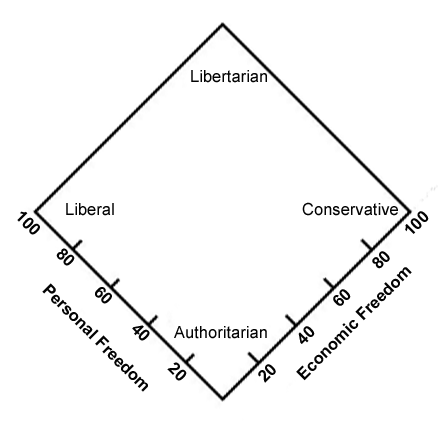
\includegraphics[width=0.7\linewidth]{1}
\end{figure}
\switchcolumn
古典自由主义者相信文明的历史是自由不断扩展的历史。
而且,古典自由主义者和民粹主义者(用 “ 国家主义者”这
个词也许更妥当)的立场实际上比自由派和保守派更加坚定。
那么我们为什么不把这个图表转一个角度,以显示对自由的坚
定信念并不只是四个选项之一,而实际上是政治思想的最高目
标呢?这样,我们得到如下图表。

\begin{figure}[!htb]
\centering

\includegraphics[width=0.7\linewidth]{2}
\end{figure}
\switchcolumn*
Now we can answer the question posed a few pages back. On
the contemporary American left-right spectrum, libertarianism
is neither left nor right. Libertarians believe in individual freedom and limited government consistently, unlike either contemporary liberals or contemporary conservatives. Some
journalists say that libertarians are conservative on economic issues and liberal on social issues, but it would make more sense
to say that contemporary liberals are libertarian on (some) social
issues but statist on economic issues, whereas contemporary conservatives are libertarian on (some) economic issues but statist on social issues.
\switchcolumn
现在我们可以回答好之前提出的问题了。在当代美国的左
一右光谱上,古典自由主义既不是左也不是右。古典自由主义
坚定地相信个人自由和有限政府,既不像当代的自由派也不像
当代的保守派。有些新闻记者说古典自由主义是经济事务上的
保守派、社会事务上的自由派,但是似乎这么说更恰当一些:
当代自由派是(某些)社会问题上的成典自由主义者和经济
问题上的国家主义者,同 时 保 守 派 是 (某些)经济问题上的
古典自由主义者和社会问题上的国家主义者。

\switchcolumn*[\section{A Note on Labels: Why ``Libertarian''?\\为什么是“古典自由主义”}]
Some people say they don't like labels. After all, each of us is too
complicated to be summed up in a word, whether it's a word
like black or white, or gay or straight, or rich or poor, or an ideological term like socialist, fascist, liberal, conservative, or libertarian. But labels serve purposes; they help us to conceptualize,
they economize on words, and if our beliefs are coherent and
consistent, there probably is a label to describe them. In any
case, if you don't label your own philosophy or movement,
someone else will label it for you. (That's how the system of
human creativity and progress in a free market got labeled
``capitalism,'' a term that refers to the accumulation of money,
which happens in any economy. It was capitalism's sworn
enemy, Karl Marx, who gave the system its name.) So I'm willing to use the term ``libertarian'' to describe my political philosophy and the movement that seeks to advance it.
\switchcolumn
有的人说他们不喜欢贴标签。毕竟,我们每一个人都太复
杂 ,不能用一个词来概括。无论是黑人还是白人,同性恋还是
异性恋,穷人还是富人,或者一个意识形态的词汇,如自由
派、保守主义者、法西斯分子或者古典自由主义者,都无法概
括一个人的本质。但是标签自然有它的作用,它能帮助我们形
成清晰的概念,简化我们论述的语言。如果我们的信念是稳定
的、一致的,可能就会有一个标签来描述它们。况且在大多数
情况下,如果你不给自己的理论和行动贴一个标签的话,其他
人会替你贴上标签。(“资本主义” 这个标签就是这么产生的。
一个人们在自由市场当中进行创造和取得进步的体系被贴上
“资本主义” 的标签,而资本主义实际是指货币积累的过程,
这种积累实际上在任何经济体中都可能发生。而 “资本主义”
这个名字是其严厉批判者马克思给取的。)于是,我就希望用
“古典自由主义”这个词来描述我的政治理论和试图推广这种
理论的运动。
\switchcolumn*
Why would anyone choose such an awkward term as libertarian to describe a political philosophy? It's a clunky neologism with too many syllables. It probably wouldn't be anyone's
first choice. But there's a historical reason for the word.

\switchcolumn
为什么有人会用古典自由主义这样拗口的词来描述一种政治理论?这是一个生造的新词,音节过多。这个词不会是人们给自己的政治观点寻找合适词汇时的第一选择。但这个词的产生有它的历史原因。
\switchcolumn*
Elements of libertarianism can be traced as far back as the
ancient Chinese philosopher Lao-tzu and the higher-law concept of the Greeks and the Israelites. In seventeenth-century
England, libertarian ideas began to take modern form in the
writings of the Levellers and John Locke. In the middle of that
century, opponents of royal power began to be called Whigs, or
sometimes simply opposition or country (as opposed to court)
writers.
\switchcolumn
古典自由主义原理的渊源,最远我们可以追溯到中国古代
的理论家老子,以及古希腊和以色列人“更高的法”(higher
-law)的观念。在 17世纪的英国,随着平权派\footnote{平权派(Levellers)是 17世纪英国内战期间的一般政治运动,主张人民主权、扩大投票权利、法律面前人人平等和宗教宽容,其观点集中表达在《人民公约》(greement of the People) 的宣言中。}和约翰$\cdot$洛克的著作的诞生,古典自由主义开始拥有了现代的形态。在17世纪中期,反对国王权力的政治人物开始被称作辉格党人,甚至那些在野的反对派和住在乡村的反对宫廷势力的作家们也被称作辉格党人。
\switchcolumn
In the 1820s the representatives of the middle class in the
Spanish Cortes, or parliament, came to be called the Liberates.
They contended with the Serviles (the servile ones), who represented the nobles and the absolute monarchy. The term
Serviles, for those who advocate state power over individuals,
unfortunately didn't stick. But the word liberal, for the defenders of liberty and the rule of law, spread rapidly. The Whig
Party in England came to be called the Liberal Party. Today we
know the philosophy of John Locke, Adam Smith, Thomas Jefferson, and John Stuart Mill as liberalism.
\switchcolumn
19世纪20年代,西班牙国会里的中产阶级代表开始被称
作 自 由 党 (Liberales)。他们和代表贵族和绝对君主权力的保
皇 党 人 (Serviles)进行斗争。保皇党一词,指的是那些拥护
国家对个人的绝对权力的人,非常贴切,不幸的是后来渐渐不
用了。但是自由党这个词,意思是维护自由和法治的人,很快
传播开来。英国的辉格党人开始被称作自由党。今天我们知道
的洛克、亚 当 $\cdot$ 斯密、杰斐逊以及密尔的理论被称作自由
主义。
\switchcolumn*
But around 1900 the term liberal underwent a change. People who supported big government and wanted to limit and
control the free market started calling themselves liberals. The
economist Joseph Schumpeter noted, ``As a supreme, if unintended, compliment, the enemies of private enterprise have
thought it wise to appropriate its label.'' Thus we now refer to
the philosophy of individual rights, free markets, and limited
government---the philosophy of Locke, Smith, and Jefferson---
as classical liberalism.
\switchcolumn
但是到20世纪初期,自由主义者这个词的含义发生了改
变。那些支持大政府、希望限制和控制自由市场的人开始自称
自由主义者。经济学家熊彼特说:“ (自由主义)成为至高的
赞誉,于是私人企业的敌人认为占用这个标签是明智的。”于
是我们现在把支持个人权利、自由市场和有限政府的理论,把洛克、亚 当 $\cdot$ 斯密和杰斐逊的理论称作传统的自由主义。
\switchcolumn*
But classical liberalism is not much of a name for a modern
political philosophy. ``Classical'' sounds old, outdated, and
carved in stone. (And in this era of historical illiteracy, if you call
yourself a classical liberal, most people think you're an admirer
of Teddy Kennedy!) Some advocates of limited government
began using the name of their old adversaries, ``conservative.''
But conservatism properly understood signifies, if not a defense
of absolute monarchy and the old order, at least an unwillingness to change and a desire to preserve the status quo. It would
be odd to refer to free-market capitalism---the most progressive, dynamic, and ever-changing system the world has ever
known---as conservative. Edward H. Crane has proposed that
today's heirs of Locke and Smith call themselves ``market liberals,'' retaining the word liberal, with its etymological connection with liberty, but reaffirming the liberal commitment to
markets. That term has been well received by market-liberal intellectuals, but it seems unlikely to catch on with journalists
and the public.
\switchcolumn
但是传统的自由主义并不像是一个现代的政治理论。“传
统” 这个词听上去老旧、过时,好像已经被刻在了碑上。而
且 ,在这个充斥了历史盲的时代,如果你称自己为传统的自由
主义,大多数人会认为你崇拜特迪$\cdot$ 肯尼迪\footnote{爱德华$\cdot$肯尼迪 (Edward  M. Kennedy), 民主党参议员,从 1962年当选	参议员至今,是参议院第二资深的议员。他 是 “ 已故的肯尼迪总统最小的弟弟,在政治上被认为是自由派。反战,主张经济、福利上的社会主义。” “特迪” 是他的昵称。} (Teddy  Kennedy) 呢! 一些有限政府的拥护者开始用以前的政治对手的称号 “保守主义者” 来称呼自己。但是对保守主义的正确理解至关重要,即便保守主义不是指拥护绝对的君主制和旧秩序的话 ,至少也应该是指保持现状、不希望改革。把自由市场资本主义这种世界上迄今为止最富有进取心、最有活力的、变化最迅速的制度称作保守主义就显得很怪异。爱德华 $\cdot$ 克兰提出,洛克和亚当$\cdot$ 斯密的思想在当代的继承人应该称作“市场自由主义”,保留了 “ 自由主义” 这个词,保持了与自由这个词
的本意的联系,但是重申对市场自由的追求。这个词巳经被自
由市场知识分子所广泛接受,但是似乎新闻界和公众的称呼还
并没有转过来。
\switchcolumn*
The right term for the advocates of civil society and free markets is arguably \textit{socialist}. Thomas Paine distinguished between society and government, and the libertarian writer Albert Jay
Nock summed up all the things that people do voluntarily---for
love or charity or profit---as ``social power,'' which is always
being threatened by the encroachment of state power. So we
might say that those who advocate social power are socialists,
while those who support state power are statists. But alas, the
word socialist, like the word liberal, has been claimed by those
who advocate neither civil society nor liberty.
\switchcolumn
其实对市民社会和自由市场的拥护者恰当的称呼应该是\textbf{社
会主义者}。这一点当然争议很大。潘恩清楚地区分了社会和政
府 ,古典自由主义作家诺克\footnote{阿尔伯特$\cdot$杰伊$\cdot$诺克(Albert Jay Nock, 1872$\sim$1945) , 美国古典自由主义思想家、教育理论家、社会批评家。}把所有人们为爱、慈善或利润而做的自愿的努力称作“社会权力”,而这常常受到国家权力的侵犯和威胁。因此,我们也许可以把那些支持社会权力的人称作社会主义者,而把那些支持国家权力的人称作国家主义者。但是遗憾的是,社会主义这个词和自由主义一样,被那些既不拥护市民社会也不拥护自由的家伙霸占了。
\switchcolumn*
In much of the world, the advocates of liberty are still called
liberals. In South Africa the liberals, such as Helen Suzman, rejected the system of racism and economic privilege known as
apartheid in favor of human rights, nonracial policies, and free
markets. In Iran liberals oppose the theocratic state and press
for Western-style ``democratic capitalism.'' In China and Russia
liberals are those who want to replace totalitarianism in all its
aspects with the classical liberal system of free markets and constitutional government. Even in Western Europe, liberal still
indicates at least a fuzzy version of classical liberalism. German
liberals, for instance, usually to be found in the Free Democratic Party, oppose the socialism of the Social Democrats, the corporatism of the Christian Democrats, and the paternalism of
both. Outside the United States, even American journalists understand the traditional meaning of liberal. In 1992, a \textit{Washington Post} story datelined Moscow reported that ``liberal
economists have criticized the government for failing to move
quickly enough with structural reforms and for allowing
money-losing state factories to continue churning out goods
that nobody needs.'' Liberal economists such as Milton Friedman make similar criticisms in the United States, but then the
Post calls them conservative economists.
\switchcolumn
而在这个世界的其他很多地方,自由的拥护者还仍然被称
作自由主义者。在南非,自 由 主 义 者 如 苏 斯 曼 (Helen  Suzman),反对种族主义和保护经济特权的种族隔离制度,争取
人权、种族平等和自由市场。在伊朗,自由主义者反对神权国
家,要求西方式的“民主资本主义”。在俄国,自由主义者是
那些要求用古典自由主义的自由市场和宪政政府来在社会各个
方面替代全权主义的人。甚至在西欧,自由主义者仍然多少有
古典自由主义的影子。实际上,德国的自由主义者大多数都是
自由民主党人,他们反对社会主义和社会民主党的政策,反对
基督教民主党的社团主义,反对这两个政党的家长权威主义。
甚至美国新闻记者到了国外,也会理解自由主义的传统含义。
例如,1992年, 《华盛顿邮报》 发自莫斯科的一篇报道称,
“ 自由主义知识分子批评政府没有很快开始体制改革,仍然让
亏损的国有企业继续生产人们不需要的产品。” 自由主义知识
分子如米尔顿$\cdot$ 弗里德曼对美国政府提出了类似的批评,但是
《华盛顿邮报》却称他们为保守主义经济学家。
\switchcolumn*
Here at home, though, by the 1940s the word liberal had
clearly been lost to the advocates of big government. Some classical liberals resisted for a time, doggedly insisting that they
were the true liberals and that the so-called liberals in Washington were in fact recreating the old order of state power that liberals had fought to overthrow. But others resigned themselves
to finding a new term. In the 1950s Leonard Read, founder of
the Foundation for Economic Education, began calling himself
a libertarian. That word had long been used for the advocates of
free will (as opposed to determinism); and, like liberal, it was
derived from the Latin \textit{liber} (free). The name was gradually embraced by a growing band of libertarians in the 1960s and
1970s. A Libertarian Party was formed in 1972. The term was
still rejected by some of the greatest twentieth-century libertarians, including Ayn Rand, who called herself a ``radical for capitalism,'' and Friedrich Hayek, who continued to call himself a
liberal or an Old Whig.
\switchcolumn
在美国,尽管到1940年代自由主义者这个词已经很明显
被大政府的支持者所霸占。一些古典自由主义者仍然抗争了很
长时间,顽强地坚持他们才是真正的自由主义者,而那些华盛
顿 的 所 谓 “ 自由主义者” 实际上是在复辟国家权力的旧秩序,
而那个旧秩序是曾经经过一代又一代自由主义者努力斗争所推
翻的。但是其他人已经放弃努力,转而寻找其他新词汇。50年代,里德(Leonard  Read),经济教育基金会(FEE)的创
始人,开 始 自 称 “古典自由主义者” (Libertarian)。这个词曾经在很长时间内被自由意志(相对于决定论)的拥护者所使
用;像自由主义这个词一样,它源于拉丁语\textit{liber}(自由)。这
个名字在60年代和70年代逐渐被越来越多的古典自由主义者
所使用。1972年还成立了一个美国自由党。这个词被一些20世纪最伟大的古典自由主义者所拒绝使用,其中包括安$\cdot$兰德(Ayn Rand), 她 自 称 “资本主义激进派”,哈耶克则继续自称
自由主义者或者“ 一个老辉格党人”。
\switchcolumn*
In this book I accept the contemporary usage. I call the ideas
I advocate, and the movement that seeks to advance them, libertarianism. Libertarianism may be regarded as a political philosophy that applies the ideas of classical liberalism consistently,
following liberal arguments to conclusions that would limit the
role of government more strictly and protect individual freedom more fully than other classical liberals would. Most of the
time, I use liberal in its traditional sense; I call today's misnamed liberals welfare-state liberals or social democrats. And I
should note that libertarian ideas and the libertarian movement
are far broader than any political party, such as the Libertarian
Party. References to libertarianism should not be taken to indicate the Libertarian Party unless that is made explicit.
\switchcolumn
本书当中我接受当代的用法。我称我拥护的理念以及推
广这种理念的运动为古典自由主义。古典自由主义也许应当
被看作是坚持实践自由主义理念的政治理论,遵行自由主义
的关于更严厉限制政府权力、更全面保护个人自由的理论,
但比其他自由主义者更加坚定。大多数时候,我使用自由主
义者这个词的时候是按照其传统的内涵来用的。我把现在的
这些被错误命名的“ 自由主义者” 称作福利主义自由派,或
者社会民主党。我将会提到,古典自由主义的理念以及实践
比任何其他政党包括美国自由党(Libertarian Party) 更加广
泛。需要指出的是,古典自由主义不等同于美国自由党,除
非我在文中特别注明。
\switchcolumn*
The old ideologies have been tried and found wanting. All
around us---from the postcommunist world to the military dictatorships of Africa to the faltering, bankrupt welfare states of
Europe and North and South America---we see the failed
legacy of coercion and statism. At the same time we see moves
toward libertarian solutions---constitutional government in Eastern Europe and South Africa, privatization in Britain and
Latin America, democracy and the rule of law in Korea and Taiwan, and demands for tax reduction everywhere. We even see
people in many parts of the world---Quebec, Croatia, Bosnia,
northern Italy, Scotland, and much of Africa, not to mention
the fifteen new republics of the old Soviet Union---challenging
the large, intrusive, incorrigible nation-states that they find
themselves in and demanding devolution of power. Libertarianism offers an alternative to coercive government that should appeal to peaceful, productive people everywhere.
\switchcolumn
旧的意识形态被不断尝试,不断被发现笨拙低效。在我们
身边,从苏东国家非洲的军事独裁政权,到欧洲、北美和南美
的步履蹒跚、财政破产的福利国家,我们都见证了强制和国家
主义遗产的失败。与此同时,我们看到通向古典自由主义的解
决方案纷纷实施 --- 东欧和南非的宪政政府的建立,英国和拉
美的私有化进程,韩国的民主化和法治的建立,以及在几乎每
一个地方都存在的减税的呼声。我们甚至在世界的许多地方
--- 魁北克、克罗地亚、波斯尼亚、北意大利、苏格兰以及非
洲的许多地方、原苏联的十五个新生的共和国 --- 看到对庞大的、专横的、压制性、不可反对的民族国家的挑战,国家权力
在不断退缩。古典自由主义对强制性制度提供了一种替代性选
择 ,这种国家将会吸引来自每一个地方的和平的人民和生
产者。
\switchcolumn*
No, a libertarian world won't be a perfect one. There will still
be inequality, poverty, crime, corruption, man's inhumanity to
man. But unlike the theocratic visionaries, the pie-in-the-sky
socialist Utopians, or the starry-eyed Mr. Fixits of the New Deal
and Great Society, libertarians don't promise you a rose garden.
Karl Popper once said that attempts to create heaven on earth
invariably produce hell. Libertarianism holds out the goal not of
a perfect society but of a better and freer one. It promises a
world in which more of the decisions will be made in the right
way by the right person: you. The result will be not an end to
crime and poverty and inequality but less---often much less---
of most of those things most of the time.
\switchcolumn
不过,古典自由主义的世界也不会是一个完美的世界。这
里仍然存在不平等、贫困、犯罪、腐败以及人与人之间的野蛮
行为。不过,与那些宗教空想主义者、天上掉馅饼式的社会主
义乌托邦,或者那些推行新政和“伟大社会” 的 幻 想 家 “改
造先生们” 不一样,古典自由主义者不会给你承诺一个玫瑰
花园。卡 尔 $\cdot$ 波普尔曾经说过,企图在地上建立天堂的努力无
一例外地会制造出地狱。古典自由主义的目标不是建立一个完
美社会,而是建立一个更好和更自由的社会。它的目标是让正
当的人用正当的方式进行决策,所谓正当的人,那就是你。其
结果不会是一个没有犯罪、贫困和不平等的社会,但会是一个
比古往今来绝大多数时候更少犯罪、贫困和不平等的社会。
\end{paracol}